\begin{figure}[t!]
  \centering

  \begin{minipage}[t]{0.49\textwidth}
    \vspace*{0pt}
    \centering
    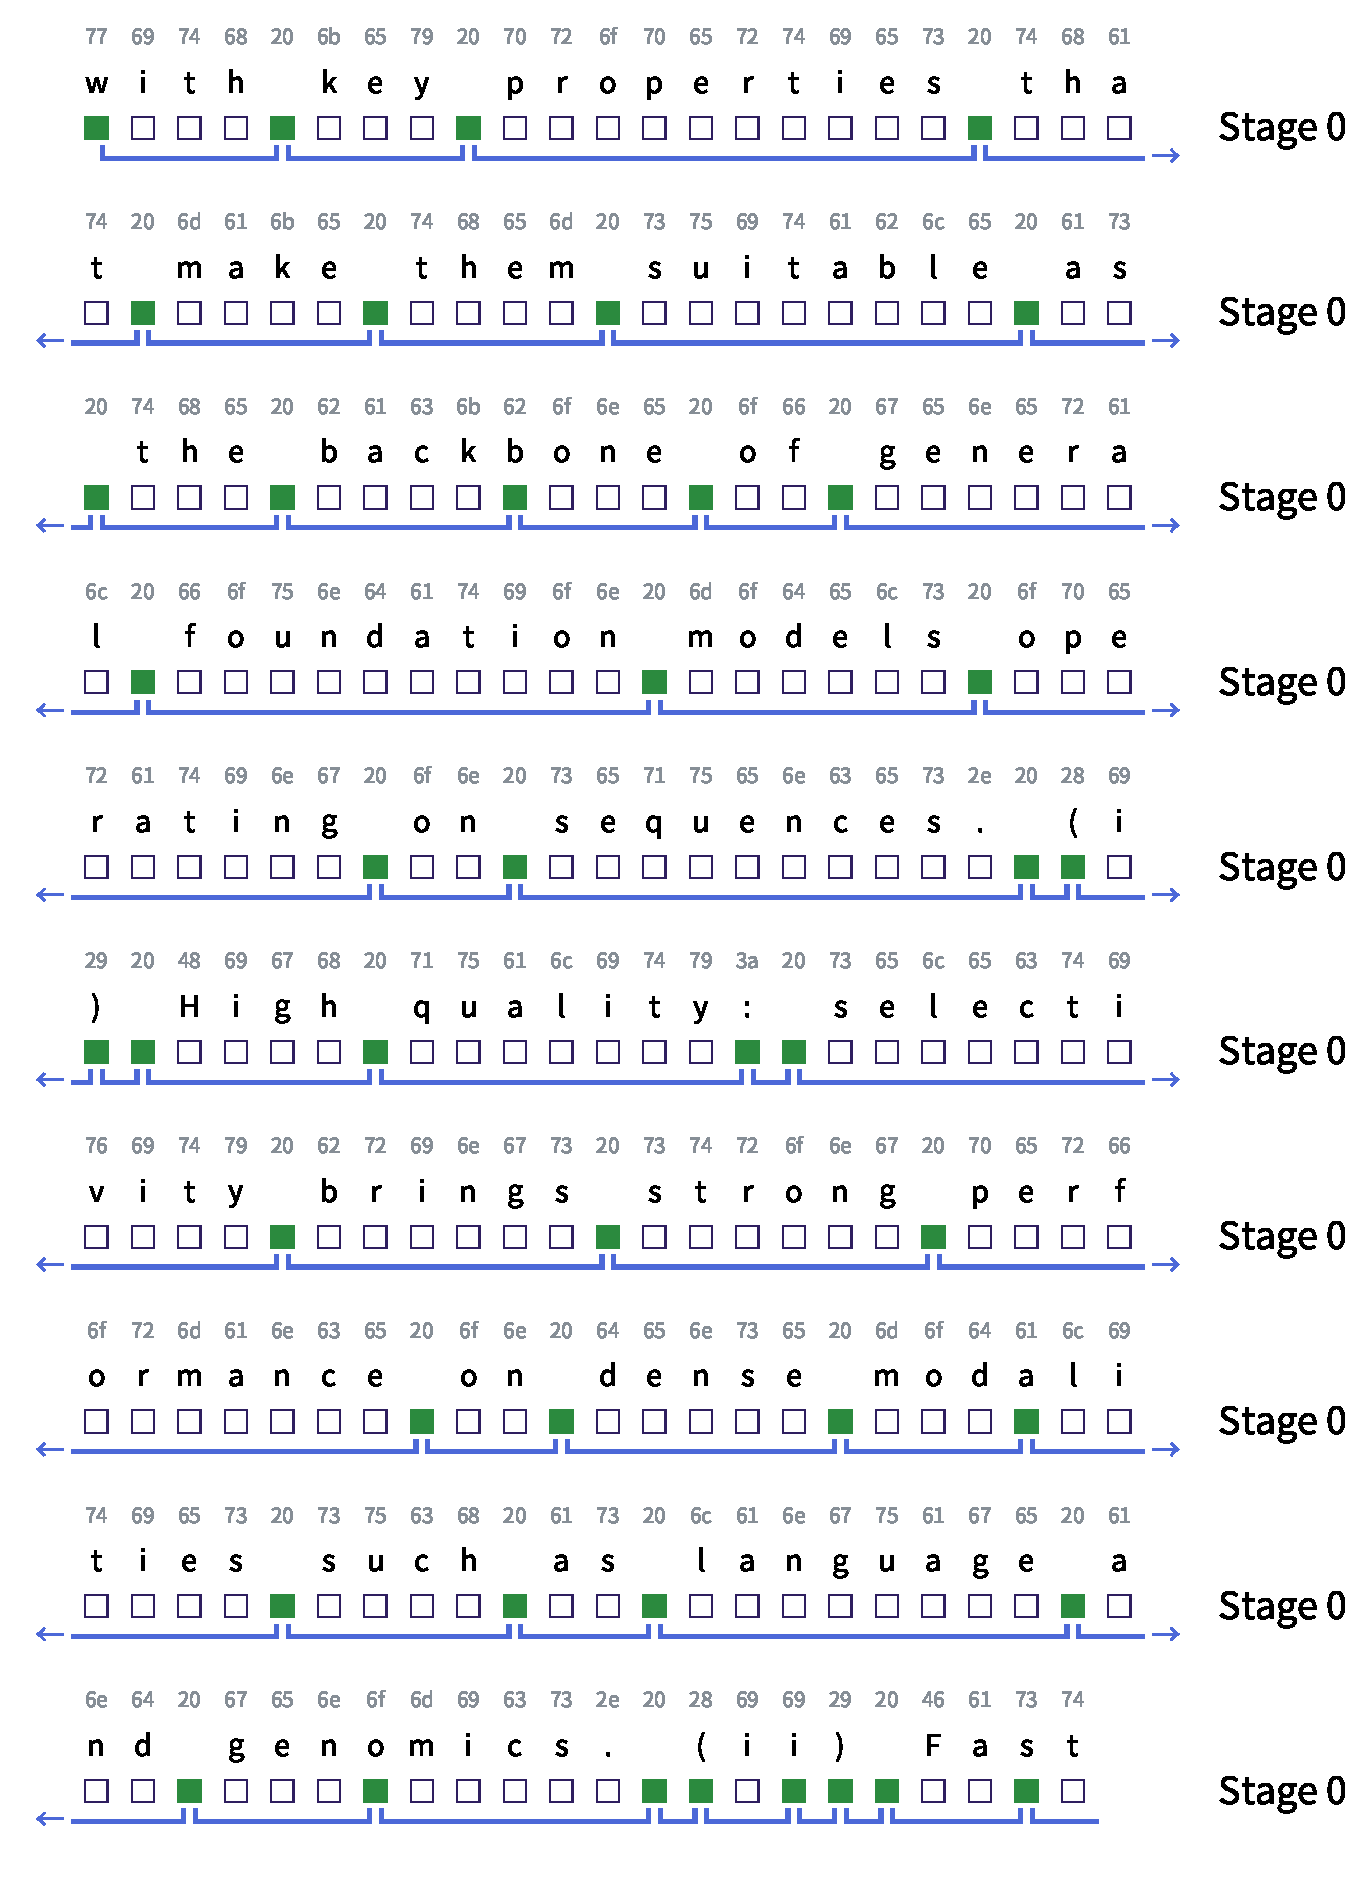
\includegraphics[width=\linewidth]{fig_img/one_stage.pdf}
    \vspace{-7mm}
    \caption*{(a) H-Net (1-stage), using $6$-DC.}

    \vspace{0pt plus 1fil}  

    \vspace{3mm}
    \captionof{figure}{
    \textbf{Visualization of boundaries drawn by H-Net.}
    Numbers above indicate byte value,
    and the colored boxes indicate positions where $b_t = 1$.
    \textbf{(a)} H-Net (1-stage) tends to draw boundaries at spacelike bytes, which is very similar to SpaceByte.
    \textbf{(b)} The boundaries of the first stage in H-Net (2-stage) are focused on spacelike bytes, as well as starting characters of each word.
    The second stage of H-Net (2-stage) chunks the text into more meaningful units, such as words or numberings (\ie{} \texttt{`(ii)'}).
    We can also observe that it often chunks multiple words that form one semantic group; for example, \texttt{`the backbone'} and \texttt{`such as'}.
    }
    \label{fig: tokenized_positions}
  \end{minipage}
  \hfill
  \begin{minipage}[t]{0.49\textwidth}
    \vspace*{0pt}
    \centering
    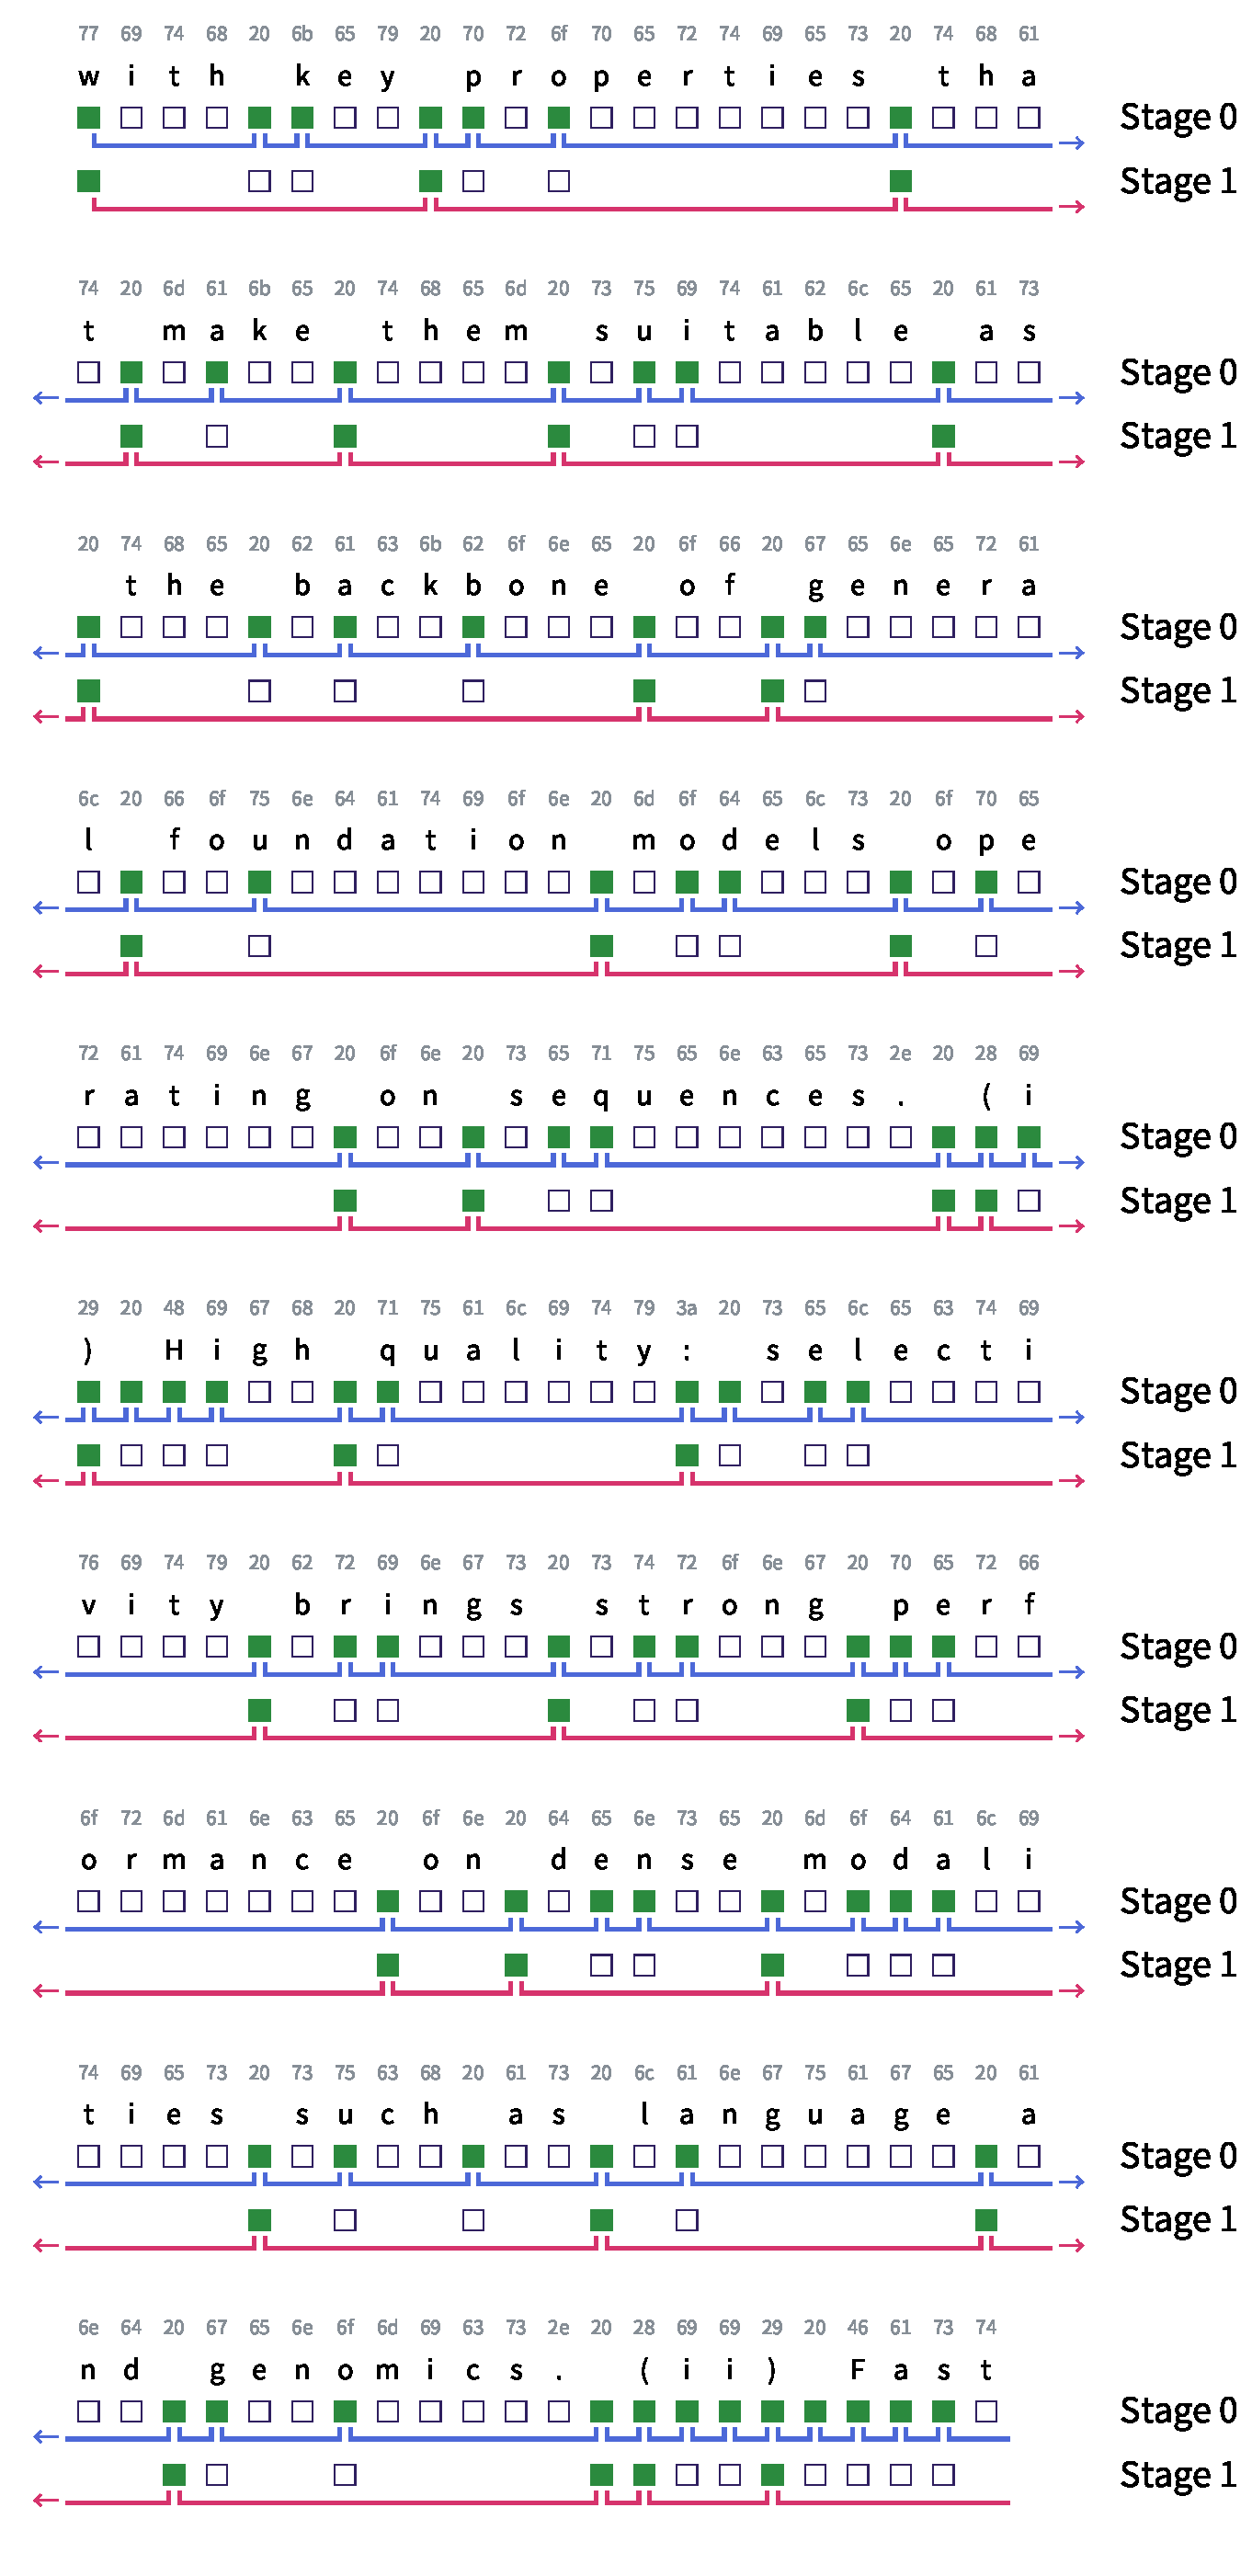
\includegraphics[width=\linewidth]{fig_img/two_stage.pdf}
    \vspace{-7mm}
    \caption*{(b) H-Net (2-stage), using (3,3)-DC.}
  \end{minipage}

\end{figure}